\documentclass[]{book}
\usepackage{lmodern}
\usepackage{amssymb,amsmath}
\usepackage{ifxetex,ifluatex}
\usepackage{fixltx2e} % provides \textsubscript
\ifnum 0\ifxetex 1\fi\ifluatex 1\fi=0 % if pdftex
  \usepackage[T1]{fontenc}
  \usepackage[utf8]{inputenc}
\else % if luatex or xelatex
  \ifxetex
    \usepackage{mathspec}
  \else
    \usepackage{fontspec}
  \fi
  \defaultfontfeatures{Ligatures=TeX,Scale=MatchLowercase}
\fi
% use upquote if available, for straight quotes in verbatim environments
\IfFileExists{upquote.sty}{\usepackage{upquote}}{}
% use microtype if available
\IfFileExists{microtype.sty}{%
\usepackage{microtype}
\UseMicrotypeSet[protrusion]{basicmath} % disable protrusion for tt fonts
}{}
\usepackage[margin=1in]{geometry}
\usepackage{hyperref}
\hypersetup{unicode=true,
            pdftitle={Statistiques et Probabilités avec R et le Tidyverse},
            pdfauthor={Marc-André Désautels},
            pdfborder={0 0 0},
            breaklinks=true}
\urlstyle{same}  % don't use monospace font for urls
\usepackage{natbib}
\bibliographystyle{apalike}
\usepackage{color}
\usepackage{fancyvrb}
\newcommand{\VerbBar}{|}
\newcommand{\VERB}{\Verb[commandchars=\\\{\}]}
\DefineVerbatimEnvironment{Highlighting}{Verbatim}{commandchars=\\\{\}}
% Add ',fontsize=\small' for more characters per line
\usepackage{framed}
\definecolor{shadecolor}{RGB}{248,248,248}
\newenvironment{Shaded}{\begin{snugshade}}{\end{snugshade}}
\newcommand{\AlertTok}[1]{\textcolor[rgb]{0.94,0.16,0.16}{#1}}
\newcommand{\AnnotationTok}[1]{\textcolor[rgb]{0.56,0.35,0.01}{\textbf{\textit{#1}}}}
\newcommand{\AttributeTok}[1]{\textcolor[rgb]{0.77,0.63,0.00}{#1}}
\newcommand{\BaseNTok}[1]{\textcolor[rgb]{0.00,0.00,0.81}{#1}}
\newcommand{\BuiltInTok}[1]{#1}
\newcommand{\CharTok}[1]{\textcolor[rgb]{0.31,0.60,0.02}{#1}}
\newcommand{\CommentTok}[1]{\textcolor[rgb]{0.56,0.35,0.01}{\textit{#1}}}
\newcommand{\CommentVarTok}[1]{\textcolor[rgb]{0.56,0.35,0.01}{\textbf{\textit{#1}}}}
\newcommand{\ConstantTok}[1]{\textcolor[rgb]{0.00,0.00,0.00}{#1}}
\newcommand{\ControlFlowTok}[1]{\textcolor[rgb]{0.13,0.29,0.53}{\textbf{#1}}}
\newcommand{\DataTypeTok}[1]{\textcolor[rgb]{0.13,0.29,0.53}{#1}}
\newcommand{\DecValTok}[1]{\textcolor[rgb]{0.00,0.00,0.81}{#1}}
\newcommand{\DocumentationTok}[1]{\textcolor[rgb]{0.56,0.35,0.01}{\textbf{\textit{#1}}}}
\newcommand{\ErrorTok}[1]{\textcolor[rgb]{0.64,0.00,0.00}{\textbf{#1}}}
\newcommand{\ExtensionTok}[1]{#1}
\newcommand{\FloatTok}[1]{\textcolor[rgb]{0.00,0.00,0.81}{#1}}
\newcommand{\FunctionTok}[1]{\textcolor[rgb]{0.00,0.00,0.00}{#1}}
\newcommand{\ImportTok}[1]{#1}
\newcommand{\InformationTok}[1]{\textcolor[rgb]{0.56,0.35,0.01}{\textbf{\textit{#1}}}}
\newcommand{\KeywordTok}[1]{\textcolor[rgb]{0.13,0.29,0.53}{\textbf{#1}}}
\newcommand{\NormalTok}[1]{#1}
\newcommand{\OperatorTok}[1]{\textcolor[rgb]{0.81,0.36,0.00}{\textbf{#1}}}
\newcommand{\OtherTok}[1]{\textcolor[rgb]{0.56,0.35,0.01}{#1}}
\newcommand{\PreprocessorTok}[1]{\textcolor[rgb]{0.56,0.35,0.01}{\textit{#1}}}
\newcommand{\RegionMarkerTok}[1]{#1}
\newcommand{\SpecialCharTok}[1]{\textcolor[rgb]{0.00,0.00,0.00}{#1}}
\newcommand{\SpecialStringTok}[1]{\textcolor[rgb]{0.31,0.60,0.02}{#1}}
\newcommand{\StringTok}[1]{\textcolor[rgb]{0.31,0.60,0.02}{#1}}
\newcommand{\VariableTok}[1]{\textcolor[rgb]{0.00,0.00,0.00}{#1}}
\newcommand{\VerbatimStringTok}[1]{\textcolor[rgb]{0.31,0.60,0.02}{#1}}
\newcommand{\WarningTok}[1]{\textcolor[rgb]{0.56,0.35,0.01}{\textbf{\textit{#1}}}}
\usepackage{longtable,booktabs}
\usepackage{graphicx,grffile}
\makeatletter
\def\maxwidth{\ifdim\Gin@nat@width>\linewidth\linewidth\else\Gin@nat@width\fi}
\def\maxheight{\ifdim\Gin@nat@height>\textheight\textheight\else\Gin@nat@height\fi}
\makeatother
% Scale images if necessary, so that they will not overflow the page
% margins by default, and it is still possible to overwrite the defaults
% using explicit options in \includegraphics[width, height, ...]{}
\setkeys{Gin}{width=\maxwidth,height=\maxheight,keepaspectratio}
\IfFileExists{parskip.sty}{%
\usepackage{parskip}
}{% else
\setlength{\parindent}{0pt}
\setlength{\parskip}{6pt plus 2pt minus 1pt}
}
\setlength{\emergencystretch}{3em}  % prevent overfull lines
\providecommand{\tightlist}{%
  \setlength{\itemsep}{0pt}\setlength{\parskip}{0pt}}
\setcounter{secnumdepth}{5}
% Redefines (sub)paragraphs to behave more like sections
\ifx\paragraph\undefined\else
\let\oldparagraph\paragraph
\renewcommand{\paragraph}[1]{\oldparagraph{#1}\mbox{}}
\fi
\ifx\subparagraph\undefined\else
\let\oldsubparagraph\subparagraph
\renewcommand{\subparagraph}[1]{\oldsubparagraph{#1}\mbox{}}
\fi

%%% Use protect on footnotes to avoid problems with footnotes in titles
\let\rmarkdownfootnote\footnote%
\def\footnote{\protect\rmarkdownfootnote}

%%% Change title format to be more compact
\usepackage{titling}

% Create subtitle command for use in maketitle
\newcommand{\subtitle}[1]{
  \posttitle{
    \begin{center}\large#1\end{center}
    }
}

\setlength{\droptitle}{-2em}
  \title{Statistiques et Probabilités avec R et le Tidyverse}
  \pretitle{\vspace{\droptitle}\centering\huge}
  \posttitle{\par}
  \author{Marc-André Désautels}
  \preauthor{\centering\large\emph}
  \postauthor{\par}
  \predate{\centering\large\emph}
  \postdate{\par}
  \date{2018-04-05}

\usepackage{booktabs}

\usepackage{amsthm}
\newtheorem{theorem}{Theorem}[chapter]
\newtheorem{lemma}{Lemma}[chapter]
\theoremstyle{definition}
\newtheorem{definition}{Definition}[chapter]
\newtheorem{corollary}{Corollary}[chapter]
\newtheorem{proposition}{Proposition}[chapter]
\theoremstyle{definition}
\newtheorem{example}{Example}[chapter]
\theoremstyle{definition}
\newtheorem{exercise}{Exercise}[chapter]
\theoremstyle{remark}
\newtheorem*{remark}{Remark}
\newtheorem*{solution}{Solution}
\begin{document}
\maketitle

{
\setcounter{tocdepth}{1}
\tableofcontents
}
\hypertarget{introduction}{%
\chapter*{Introduction}\label{introduction}}
\addcontentsline{toc}{chapter}{Introduction}

\hypertarget{part-pourquoi-le-tidyverse}{%
\part{Pourquoi le
tidyverse}\label{part-pourquoi-le-tidyverse}}

\hypertarget{tidyverse}{%
\chapter{Le tidyverse}\label{tidyverse}}

Dans ce document, nous utiliserons l'extension \texttt{tidyverse} par
\citep{R-tidyverse}. Ce chapitre permettra d'introduire l'extension
\texttt{tidyverse} mais surtout les principes qui la sous-tendent. Ce
chapitre est inspiré de \citep{juba2018} et \citep{wickham2017}.

\begin{Shaded}
\begin{Highlighting}[]
\KeywordTok{library}\NormalTok{(tidyverse)}
\KeywordTok{library}\NormalTok{(questionr)}
\end{Highlighting}
\end{Shaded}

\hypertarget{extensions}{%
\section{Extensions}\label{extensions}}

Le terme \emph{tidyverse} est une contraction de \emph{tidy} (qu'on
pourrait traduire par ``bien rangé'') et de \emph{universe}. En allant
visiter le site internet de ces extensions
\url{https://www.tidyverse.org/}, voici ce que nous pouvons trouver sur
la première page du site:

\begin{quote}
The tidyverse is an opinionated collection of R packages designed for
data science. All packages share an underlying design philosophy,
grammar, and data structures.
\end{quote}

que nous pourrions traduire par:

\begin{quote}
Le tidyverse est une collection dogmatique d'extensions pour le langage
R conçues pour la science des données. Toutes les extensions partagent
une philosphie sous-jacente de design, de grammaire et de structures de
données.
\end{quote}

Ces extensions abordent un très grand nombre d'opérations courantes dans
\texttt{R}. L'avantage d'utiliser le \texttt{tidyverse} c'est qu'il
permet de simplifier plusieurs opérations fréquentes et il introduit le
concept de \textbf{tidy data}. De plus, la grammaire du
\texttt{tidyverse} étant cohérente entre toutes ses extensions, en
apprenant comment utiliser l'une de ces extensions, vous serez en monde
connu lorsque viendra le temps d'apprendre de nouvelles extensions.

Nous utiliserons le \texttt{tidyverse} pour:

\begin{itemize}
\tightlist
\item
  Le concept de \textbf{tidy data}
\item
  L'importation et/ou l'exportation de données
\item
  La manipulation de variables
\item
  La visualisation
\end{itemize}

Le \texttt{tidyverse} permet aussi de:

\begin{itemize}
\tightlist
\item
  Travailler avec des chaînes de caractères (du texte par exemple)
\item
  Programmer
\item
  Remettre en forme des données
\item
  Extraire des données du Web
\item
  Etc.
\end{itemize}

Pour en savoir plus, nous invitons le lecteur à se rendre au site du
\texttt{tidyverse} \url{https://www.tidyverse.org/}. Le
\texttt{tidyverse} est en grande partie issu des travaux de
\href{http://hadley.nz/}{Hadley Wickham}.

\hypertarget{installation}{%
\section{Installation}\label{installation}}

Pour installer les extensions du \texttt{tidyverse}, nous effectuons la
commande suivante:

\begin{Shaded}
\begin{Highlighting}[]
\KeywordTok{install.packages}\NormalTok{(}\StringTok{"tidyverse"}\NormalTok{)}
\end{Highlighting}
\end{Shaded}

Une fois l'extension installée, il n'est pas nécessaire de la
réinstaller à chaque fois que vous utilisez \texttt{R}. Par contre, vous
devez charger l'extension à chaque fois que vous utilisez \texttt{R}.

Pour charger l'extension et l'utiliser dans \texttt{R}, nous effectuons
la commande suivante:

\begin{Shaded}
\begin{Highlighting}[]
\KeywordTok{library}\NormalTok{(tidyverse)}
\end{Highlighting}
\end{Shaded}

Cette commande va en fait charger plusieurs extensions qui constituent
le \textbf{coeur} du \texttt{tidyverse}, à savoir :

\begin{itemize}
\tightlist
\item
  \texttt{ggplot2} (visualisation)
\item
  \texttt{dplyr} (manipulation des données)
\item
  \texttt{tidyr} (remise en forme des données)
\item
  \texttt{purrr} (programmation)
\item
  \texttt{readr} (importation de données)
\item
  \texttt{tibble} (tableaux de données)
\item
  \texttt{forcats} (variables qualitatives)
\item
  \texttt{stringr} (chaînes de caractères)
\end{itemize}

Il existe d'autres extensions qui font partie du \texttt{tidyverse} mais
qui doivent être chargées explicitement, comme par exemple
\texttt{readxl} (pour l'importation de données depuis des fichiers
Excel).

La liste complète des extensions se trouve sur le site officiel du
\texttt{tidyverse} \url{https://www.tidyverse.org/packages/}.

\hypertarget{tidydata}{%
\section{Les tidy data}\label{tidydata}}

Le \texttt{tidyverse} est en partie fondé sur le concept de \emph{tidy
data}, développé à l'origine par Hadley Wickham dans un article du
\emph{Journal of Statistical Software}, voir \citep{wickham2014}. Nous
pourrions traduire ce concept par \emph{données bien rangées}.

Il s'agit d'un modèle d'organisation des données qui vise à faciliter le
travail souvent long et fastidieux de nettoyage et de préparation
préalable à la mise en oeuvre de méthodes d'analyse. Dans ce livre, nous
travaillerons toujours avec des \emph{tidy data}. En réalité, la plupart
des données rencontrées par les chercheurs ne sont pas \emph{tidy}. Il
existe une extension du \texttt{tidyverse} qui permet de faciliter la
transformation de données \emph{non tidy} en données \emph{tidy},
l'extension \texttt{tidyr}. Nous ne verrons pas comment l'utiliser dans
ce livre.

Les principes d'un jeu de données \emph{tidy} sont les suivants :

\begin{enumerate}
\def\labelenumi{\arabic{enumi}.}
\tightlist
\item
  chaque variable est une colonne
\item
  chaque observation est une ligne
\item
  chaque valeur doit être dans une cellule différente
\end{enumerate}

La figure \ref{fig:tidy-structure} montre ces règles de façon visuelle
(l'image a été prise de \citep{wickham2017}).

\begin{figure}

{\centering 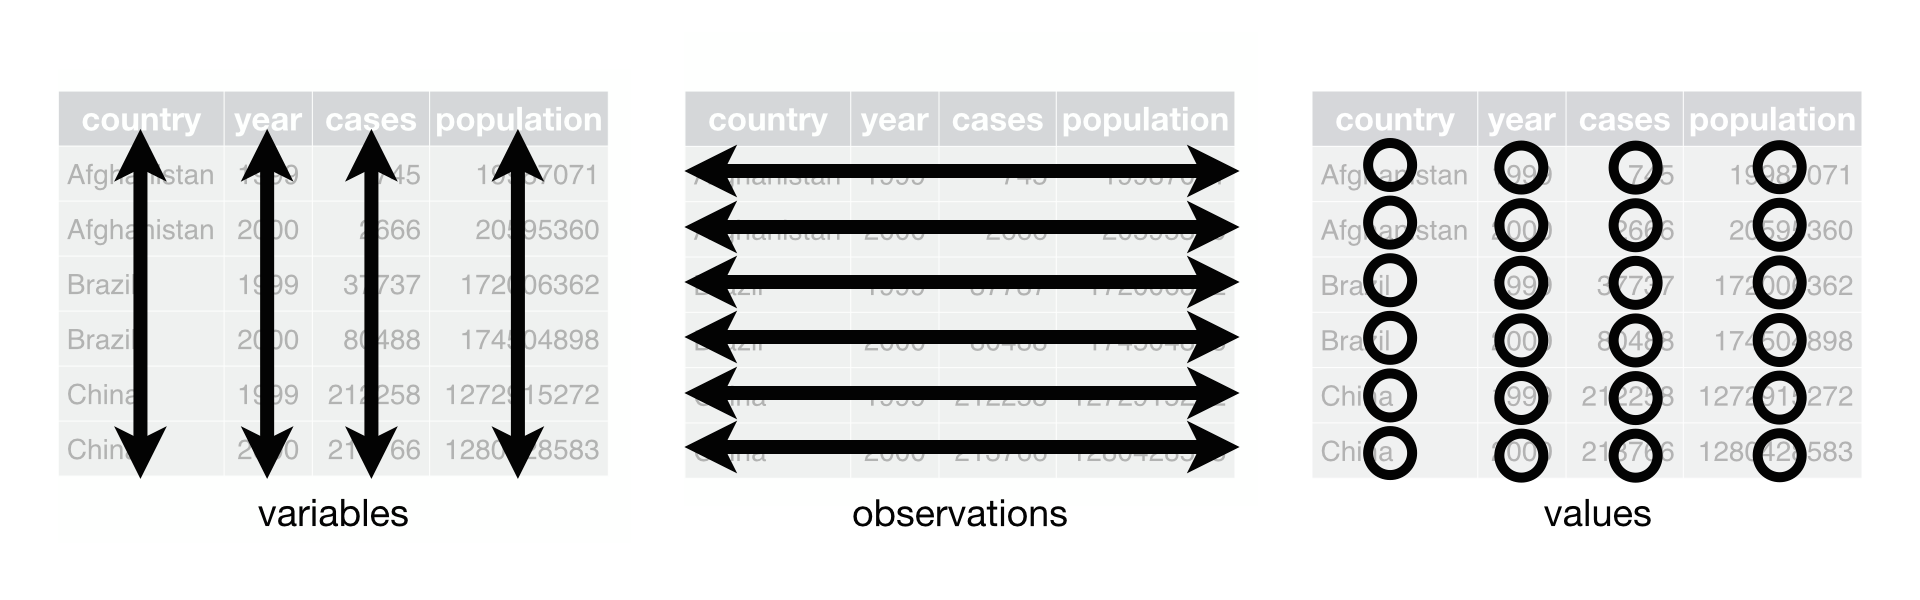
\includegraphics[width=1\linewidth]{images/tidy-1} 

}

\caption{Suivre les trois principes rend les données tidy: les variables sont en colonnes, les observations sont sur des lignes, et chaques valeurs sont dans des cellules différentes.}\label{fig:tidy-structure}
\end{figure}

Pourquoi s'assurer que vos données sont \emph{tidy}? Il y a deux
avantages importants:

\begin{enumerate}
\def\labelenumi{\arabic{enumi}.}
\item
  Un avantage général de choisir une seule façon de conserver vos
  données. Si vous utilisez une structure de données consitante, il est
  plus facile d'apprendre à utiliser les outils qui fonctionneront avec
  ce type de structure, étant donné que celles-ci possède une uniformité
  sous-jacente.
\item
  Un avantage spécifique de placer les variables en colonnes car ceci
  permet de \emph{vectoriser} les opérations dans \texttt{R}. Ceci
  implique que vos fonctions seront plus rapides lorsque viendra le
  temps de les exécuter.
\end{enumerate}

Voici un exemple de données \emph{tidy} qui sont accessibles en
\texttt{R} de base.

\begin{Shaded}
\begin{Highlighting}[]
\KeywordTok{as_tibble}\NormalTok{(}\KeywordTok{rownames_to_column}\NormalTok{(mtcars))}
\NormalTok{## # A tibble: 32 x 12}
\NormalTok{##   rowname        mpg   cyl  disp    hp  drat    wt  qsec    vs    am  gear}
\NormalTok{##   <chr>        <dbl> <dbl> <dbl> <dbl> <dbl> <dbl> <dbl> <dbl> <dbl> <dbl>}
\NormalTok{## 1 Mazda RX4     21.0    6.  160.  110.  3.90  2.62  16.5    0.    1.    4.}
\NormalTok{## 2 Mazda RX4 W~  21.0    6.  160.  110.  3.90  2.88  17.0    0.    1.    4.}
\NormalTok{## 3 Datsun 710    22.8    4.  108.   93.  3.85  2.32  18.6    1.    1.    4.}
\NormalTok{## 4 Hornet 4 Dr~  21.4    6.  258.  110.  3.08  3.22  19.4    1.    0.    3.}
\NormalTok{## 5 Hornet Spor~  18.7    8.  360.  175.  3.15  3.44  17.0    0.    0.    3.}
\NormalTok{## 6 Valiant       18.1    6.  225.  105.  2.76  3.46  20.2    1.    0.    3.}
\NormalTok{## # ... with 26 more rows, and 1 more variable: carb <dbl>}
\end{Highlighting}
\end{Shaded}

\hypertarget{tibbles}{%
\section{Les tibbles}\label{tibbles}}

Une autre particularité du \emph{tidyverse} est que ces extensions
travaillent avec des tableaux de données au format \emph{tibble}, qui
est une évolution plus moderne du classique \emph{data frame} du R de
base. Ce format est fourni est géré par l'extension du même nom
(\texttt{tibble}), qui fait partie du coeur du \emph{tidyverse}. La
plupart des fonctions des extensions du \emph{tidyverse} acceptent des
\emph{data frames} en entrée, mais retournent un objet de classe
\texttt{tibble}.

Contrairement aux \emph{data frames}, les \emph{tibbles} :

\begin{itemize}
\tightlist
\item
  n'ont pas de noms de lignes (\emph{rownames})
\item
  autorisent des noms de colonnes invalides pour les \emph{data frames}
  (espaces, caractères spéciaux, nombres\ldots{}) \footnote{Quand on
    veut utiliser des noms de ce type, on doit les entourer avec des
    \emph{backticks} (`)}
\item
  s'affichent plus intelligemment que les \emph{data frames} : seules
  les premières lignes sont affichées, ainsi que quelques informations
  supplémentaires utiles (dimensions, types des colonnes\ldots{})
\item
  ne font pas de \emph{partial matching} sur les noms de colonnes
  \footnote{Dans R de base, si une table \texttt{d} contient une colonne
    \texttt{qualif}, \texttt{d\$qual} retournera cette colonne.}
\item
  affichent un avertissement si on essaie d'accéder à une colonne qui
  n'existe pas
\end{itemize}

Pour autant, les tibbles restent compatibles avec les \emph{data
frames}. On peut ainsi facilement convertir un \emph{data frame} en
tibble avec \texttt{as\_tibble} :

\begin{Shaded}
\begin{Highlighting}[]
\KeywordTok{as_tibble}\NormalTok{(mtcars)}
\NormalTok{## # A tibble: 32 x 11}
\NormalTok{##     mpg   cyl  disp    hp  drat    wt  qsec    vs    am  gear  carb}
\NormalTok{## * <dbl> <dbl> <dbl> <dbl> <dbl> <dbl> <dbl> <dbl> <dbl> <dbl> <dbl>}
\NormalTok{## 1  21.0    6.  160.  110.  3.90  2.62  16.5    0.    1.    4.    4.}
\NormalTok{## 2  21.0    6.  160.  110.  3.90  2.88  17.0    0.    1.    4.    4.}
\NormalTok{## 3  22.8    4.  108.   93.  3.85  2.32  18.6    1.    1.    4.    1.}
\NormalTok{## 4  21.4    6.  258.  110.  3.08  3.22  19.4    1.    0.    3.    1.}
\NormalTok{## 5  18.7    8.  360.  175.  3.15  3.44  17.0    0.    0.    3.    2.}
\NormalTok{## 6  18.1    6.  225.  105.  2.76  3.46  20.2    1.    0.    3.    1.}
\NormalTok{## # ... with 26 more rows}
\end{Highlighting}
\end{Shaded}

Si le \emph{data frame} d'origine a des \emph{rownames}, on peut d'abord
les convertir en colonnes avec \texttt{rownames\_to\_columns} :

\begin{Shaded}
\begin{Highlighting}[]
\NormalTok{d <-}\StringTok{ }\KeywordTok{as_tibble}\NormalTok{(}\KeywordTok{rownames_to_column}\NormalTok{(mtcars))}
\NormalTok{d}
\NormalTok{## # A tibble: 32 x 12}
\NormalTok{##   rowname        mpg   cyl  disp    hp  drat    wt  qsec    vs    am  gear}
\NormalTok{##   <chr>        <dbl> <dbl> <dbl> <dbl> <dbl> <dbl> <dbl> <dbl> <dbl> <dbl>}
\NormalTok{## 1 Mazda RX4     21.0    6.  160.  110.  3.90  2.62  16.5    0.    1.    4.}
\NormalTok{## 2 Mazda RX4 W~  21.0    6.  160.  110.  3.90  2.88  17.0    0.    1.    4.}
\NormalTok{## 3 Datsun 710    22.8    4.  108.   93.  3.85  2.32  18.6    1.    1.    4.}
\NormalTok{## 4 Hornet 4 Dr~  21.4    6.  258.  110.  3.08  3.22  19.4    1.    0.    3.}
\NormalTok{## 5 Hornet Spor~  18.7    8.  360.  175.  3.15  3.44  17.0    0.    0.    3.}
\NormalTok{## 6 Valiant       18.1    6.  225.  105.  2.76  3.46  20.2    1.    0.    3.}
\NormalTok{## # ... with 26 more rows, and 1 more variable: carb <dbl>}
\end{Highlighting}
\end{Shaded}

À l'inverse, on peut à tout moment convertir un tibble en \emph{data
frame} avec \texttt{as.data.frame} :

\begin{Shaded}
\begin{Highlighting}[]
\KeywordTok{as.data.frame}\NormalTok{(d)}
\NormalTok{##                rowname  mpg cyl  disp  hp drat   wt qsec vs am gear carb}
\NormalTok{## 1            Mazda RX4 21.0   6 160.0 110 3.90 2.62 16.5  0  1    4    4}
\NormalTok{## 2        Mazda RX4 Wag 21.0   6 160.0 110 3.90 2.88 17.0  0  1    4    4}
\NormalTok{## 3           Datsun 710 22.8   4 108.0  93 3.85 2.32 18.6  1  1    4    1}
\NormalTok{## 4       Hornet 4 Drive 21.4   6 258.0 110 3.08 3.21 19.4  1  0    3    1}
\NormalTok{## 5    Hornet Sportabout 18.7   8 360.0 175 3.15 3.44 17.0  0  0    3    2}
\NormalTok{## 6              Valiant 18.1   6 225.0 105 2.76 3.46 20.2  1  0    3    1}
\NormalTok{## 7           Duster 360 14.3   8 360.0 245 3.21 3.57 15.8  0  0    3    4}
\NormalTok{## 8            Merc 240D 24.4   4 146.7  62 3.69 3.19 20.0  1  0    4    2}
\NormalTok{## 9             Merc 230 22.8   4 140.8  95 3.92 3.15 22.9  1  0    4    2}
\NormalTok{## 10            Merc 280 19.2   6 167.6 123 3.92 3.44 18.3  1  0    4    4}
\NormalTok{## 11           Merc 280C 17.8   6 167.6 123 3.92 3.44 18.9  1  0    4    4}
\NormalTok{## 12          Merc 450SE 16.4   8 275.8 180 3.07 4.07 17.4  0  0    3    3}
\NormalTok{## 13          Merc 450SL 17.3   8 275.8 180 3.07 3.73 17.6  0  0    3    3}
\NormalTok{## 14         Merc 450SLC 15.2   8 275.8 180 3.07 3.78 18.0  0  0    3    3}
\NormalTok{## 15  Cadillac Fleetwood 10.4   8 472.0 205 2.93 5.25 18.0  0  0    3    4}
\NormalTok{## 16 Lincoln Continental 10.4   8 460.0 215 3.00 5.42 17.8  0  0    3    4}
\NormalTok{## 17   Chrysler Imperial 14.7   8 440.0 230 3.23 5.34 17.4  0  0    3    4}
\NormalTok{## 18            Fiat 128 32.4   4  78.7  66 4.08 2.20 19.5  1  1    4    1}
\NormalTok{## 19         Honda Civic 30.4   4  75.7  52 4.93 1.61 18.5  1  1    4    2}
\NormalTok{## 20      Toyota Corolla 33.9   4  71.1  65 4.22 1.83 19.9  1  1    4    1}
\NormalTok{## 21       Toyota Corona 21.5   4 120.1  97 3.70 2.46 20.0  1  0    3    1}
\NormalTok{## 22    Dodge Challenger 15.5   8 318.0 150 2.76 3.52 16.9  0  0    3    2}
\NormalTok{## 23         AMC Javelin 15.2   8 304.0 150 3.15 3.44 17.3  0  0    3    2}
\NormalTok{## 24          Camaro Z28 13.3   8 350.0 245 3.73 3.84 15.4  0  0    3    4}
\NormalTok{## 25    Pontiac Firebird 19.2   8 400.0 175 3.08 3.85 17.1  0  0    3    2}
\NormalTok{## 26           Fiat X1-9 27.3   4  79.0  66 4.08 1.94 18.9  1  1    4    1}
\NormalTok{## 27       Porsche 914-2 26.0   4 120.3  91 4.43 2.14 16.7  0  1    5    2}
\NormalTok{## 28        Lotus Europa 30.4   4  95.1 113 3.77 1.51 16.9  1  1    5    2}
\NormalTok{## 29      Ford Pantera L 15.8   8 351.0 264 4.22 3.17 14.5  0  1    5    4}
\NormalTok{## 30        Ferrari Dino 19.7   6 145.0 175 3.62 2.77 15.5  0  1    5    6}
\NormalTok{## 31       Maserati Bora 15.0   8 301.0 335 3.54 3.57 14.6  0  1    5    8}
\NormalTok{## 32          Volvo 142E 21.4   4 121.0 109 4.11 2.78 18.6  1  1    4    2}
\end{Highlighting}
\end{Shaded}

Là encore, on peut convertir la colonne \texttt{rowname} en ``vrais''
\emph{rownames} avec \texttt{column\_to\_rownames} :

\begin{Shaded}
\begin{Highlighting}[]
\KeywordTok{column_to_rownames}\NormalTok{(}\KeywordTok{as.data.frame}\NormalTok{(d))}
\NormalTok{##                      mpg cyl  disp  hp drat   wt qsec vs am gear carb}
\NormalTok{## Mazda RX4           21.0   6 160.0 110 3.90 2.62 16.5  0  1    4    4}
\NormalTok{## Mazda RX4 Wag       21.0   6 160.0 110 3.90 2.88 17.0  0  1    4    4}
\NormalTok{## Datsun 710          22.8   4 108.0  93 3.85 2.32 18.6  1  1    4    1}
\NormalTok{## Hornet 4 Drive      21.4   6 258.0 110 3.08 3.21 19.4  1  0    3    1}
\NormalTok{## Hornet Sportabout   18.7   8 360.0 175 3.15 3.44 17.0  0  0    3    2}
\NormalTok{## Valiant             18.1   6 225.0 105 2.76 3.46 20.2  1  0    3    1}
\NormalTok{## Duster 360          14.3   8 360.0 245 3.21 3.57 15.8  0  0    3    4}
\NormalTok{## Merc 240D           24.4   4 146.7  62 3.69 3.19 20.0  1  0    4    2}
\NormalTok{## Merc 230            22.8   4 140.8  95 3.92 3.15 22.9  1  0    4    2}
\NormalTok{## Merc 280            19.2   6 167.6 123 3.92 3.44 18.3  1  0    4    4}
\NormalTok{## Merc 280C           17.8   6 167.6 123 3.92 3.44 18.9  1  0    4    4}
\NormalTok{## Merc 450SE          16.4   8 275.8 180 3.07 4.07 17.4  0  0    3    3}
\NormalTok{## Merc 450SL          17.3   8 275.8 180 3.07 3.73 17.6  0  0    3    3}
\NormalTok{## Merc 450SLC         15.2   8 275.8 180 3.07 3.78 18.0  0  0    3    3}
\NormalTok{## Cadillac Fleetwood  10.4   8 472.0 205 2.93 5.25 18.0  0  0    3    4}
\NormalTok{## Lincoln Continental 10.4   8 460.0 215 3.00 5.42 17.8  0  0    3    4}
\NormalTok{## Chrysler Imperial   14.7   8 440.0 230 3.23 5.34 17.4  0  0    3    4}
\NormalTok{## Fiat 128            32.4   4  78.7  66 4.08 2.20 19.5  1  1    4    1}
\NormalTok{## Honda Civic         30.4   4  75.7  52 4.93 1.61 18.5  1  1    4    2}
\NormalTok{## Toyota Corolla      33.9   4  71.1  65 4.22 1.83 19.9  1  1    4    1}
\NormalTok{## Toyota Corona       21.5   4 120.1  97 3.70 2.46 20.0  1  0    3    1}
\NormalTok{## Dodge Challenger    15.5   8 318.0 150 2.76 3.52 16.9  0  0    3    2}
\NormalTok{## AMC Javelin         15.2   8 304.0 150 3.15 3.44 17.3  0  0    3    2}
\NormalTok{## Camaro Z28          13.3   8 350.0 245 3.73 3.84 15.4  0  0    3    4}
\NormalTok{## Pontiac Firebird    19.2   8 400.0 175 3.08 3.85 17.1  0  0    3    2}
\NormalTok{## Fiat X1-9           27.3   4  79.0  66 4.08 1.94 18.9  1  1    4    1}
\NormalTok{## Porsche 914-2       26.0   4 120.3  91 4.43 2.14 16.7  0  1    5    2}
\NormalTok{## Lotus Europa        30.4   4  95.1 113 3.77 1.51 16.9  1  1    5    2}
\NormalTok{## Ford Pantera L      15.8   8 351.0 264 4.22 3.17 14.5  0  1    5    4}
\NormalTok{## Ferrari Dino        19.7   6 145.0 175 3.62 2.77 15.5  0  1    5    6}
\NormalTok{## Maserati Bora       15.0   8 301.0 335 3.54 3.57 14.6  0  1    5    8}
\NormalTok{## Volvo 142E          21.4   4 121.0 109 4.11 2.78 18.6  1  1    4    2}
\end{Highlighting}
\end{Shaded}

Les deux fonctions \texttt{column\_to\_rownames} et
\texttt{rownames\_to\_column} acceptent un argument supplémentaire
\texttt{var} qui permet d'indiquer un nom de colonne autre que le nom
\texttt{rowname} utilisé par défaut pour créer ou identifier la colonne
contenant les noms de lignes.

Pour être en mesure d'effectuer des calculs statistiques, il nous faut
une structure qui soit en mesure de garder en mémoire une base de
données. Ces structures se nomment des ``tibbles'' dans R.

\hypertarget{prerequis}{%
\subsection{Prérequis}\label{prerequis}}

Pour être en mesure d'utiliser le paquetage \textbf{tibble}, nous devons
charger le paquetage \textbf{tibble} et le paquetage \textbf{knitr}.
Pour ce faire, il suffit d'utiliser la commande suivante:

\begin{Shaded}
\begin{Highlighting}[]
\KeywordTok{library}\NormalTok{(tibble)}
\KeywordTok{library}\NormalTok{(knitr)}
\end{Highlighting}
\end{Shaded}

Si vous exécutez ce code et vous recevez le message d'erreur suivant
``there is no package called `tibble'\,'', vous allez devoir installer
le paquetage et ensuite charger la librairie.

\begin{verbatim}
install.packages("tibble")
library(tibble)
\end{verbatim}

Vous faites la même chose pour le paquetage \textbf{knitr}.

Vous devez installer le paquetage une seule fois, mais vous devez le
charger à chaque fois que vous démarrez une session en R.

\hypertarget{un-exemple-de-tibble}{%
\subsection{Un exemple de ``tibble''}\label{un-exemple-de-tibble}}

Pour comprendre ce qu'est un ``tibble'', nous allons utiliser deux
paquetages: ``nycflights13'' et ``diamonds''. Si ce n'est pas déjà fait,
vous devez les installer et ensuite les charger.

\begin{Shaded}
\begin{Highlighting}[]
\KeywordTok{library}\NormalTok{(nycflights13)}
\KeywordTok{library}\NormalTok{(ggplot2)}
\end{Highlighting}
\end{Shaded}

Nous allons étudier le paquetage ``nycflights13'' qui contient 5 bases
de données contenant des informations concernant les vols intérieurs en
partance de New York en 2013, à partir des aéroports de Newark Liberty
International (EWR), John F. Kennedy International (JFK) ou LaGuardia
(LGA). Les 5 bases de données sont les suivantes:

\begin{itemize}
\tightlist
\item
  flights: information sur les 336,776 vols
\item
  airlines: lien entre les codes IATA de deux lettres et les noms de
  compagnies d'aviation (16 au total)
\item
  planes: information de construction sur les 3 322 avions utilisés
\item
  weather: données météo à chaque heure (environ 8 710 observations)
  pour chacun des trois aéroports.
\item
  airports: noms des aéroports et localisations
\end{itemize}

\hypertarget{la-base-de-donnees-flights}{%
\subsection{La base de données
flights}\label{la-base-de-donnees-flights}}

Pour visualiser facilement une base de données sous forme ``tibble'', il
suffit de taper son nom dans la console. Nous allons utiliser la base de
données flights. Par exemple:

\begin{Shaded}
\begin{Highlighting}[]
\NormalTok{flights}
\NormalTok{## # A tibble: 336,776 x 19}
\NormalTok{##    year month   day dep_time sched_dep_time dep_delay arr_time}
\NormalTok{##   <int> <int> <int>    <int>          <int>     <dbl>    <int>}
\NormalTok{## 1  2013     1     1      517            515        2.      830}
\NormalTok{## 2  2013     1     1      533            529        4.      850}
\NormalTok{## 3  2013     1     1      542            540        2.      923}
\NormalTok{## 4  2013     1     1      544            545       -1.     1004}
\NormalTok{## 5  2013     1     1      554            600       -6.      812}
\NormalTok{## 6  2013     1     1      554            558       -4.      740}
\NormalTok{## # ... with 3.368e+05 more rows, and 12 more variables:}
\NormalTok{## #   sched_arr_time <int>, arr_delay <dbl>, carrier <chr>, flight <int>,}
\NormalTok{## #   tailnum <chr>, origin <chr>, dest <chr>, air_time <dbl>,}
\NormalTok{## #   distance <dbl>, hour <dbl>, minute <dbl>, time_hour <dttm>}
\end{Highlighting}
\end{Shaded}

Nous allons décortiquer la sortie console:

\begin{itemize}
\tightlist
\item
  \texttt{A\ tibble:\ 336,776\ x\ 19}: un ``tibble'' est une façon de
  représenter une base de données en R. Cette base de données possède:

  \begin{itemize}
  \tightlist
  \item
    \texttt{336\ 776} lignes
  \item
    \texttt{19} colonnes correspondant aux 19 variables décrivant
    chacune des observations
  \end{itemize}
\item
  \texttt{year\ month} \texttt{day} \texttt{dep\_time}
  \texttt{sched\_dep\_time} \texttt{dep\_delay} \texttt{arr\_time} sont
  différentes colonnes, en d'autres mots des variables, de cette base de
  données.
\item
  Nous avons ensuite 10 lignes d'obervations correspondant à 10 vols
\item
  \texttt{...\ with\ 336,766\ more\ rows,\ and\ 12\ more\ variables:}
  nous indique que 336 766 lignes et 12 autres variables ne pouvaient
  pas être affichées à l'écran.
\end{itemize}

Malheureusement cette sortie écran ne nous permet pas d'explorer les
données correctement. Nous verrons à la section \ref{explorertibbles}
comment explorer des \texttt{tibbles}.

\hypertarget{donneesdiamonds}{%
\subsection{\texorpdfstring{La base de données
\texttt{diamonds}}{La base de données diamonds}}\label{donneesdiamonds}}

La base de données \texttt{diamonds} est composée des variables
suivantes:

\begin{itemize}
\tightlist
\item
  \texttt{price} : prix en dollars US
\item
  \texttt{carat} : poids du diamant en grammes
\item
  \texttt{cut} : qualité de la coupe (Fair, Good, Very Good, Premium,
  Ideal)
\item
  \texttt{color} : couleur du diamant (J (pire) jusqu'à D (meilleur))
\item
  \texttt{clarity} : une mesure de la clarté du diamant (I1 (pire), SI2,
  SI1, VS2, VS1, VVS2, VVS1, IF (meilleur))
\item
  \texttt{x} : longueur en mm
\item
  \texttt{y} : largeur en mm
\item
  \texttt{z} : hauteur en mm
\item
  \texttt{depth} : z / mean(x, y) = 2 * z / (x + y)
\item
  \texttt{table} : largeur du dessus du diamant par rapport à son point
  le plus large
\end{itemize}

\begin{Shaded}
\begin{Highlighting}[]
\NormalTok{diamonds}
\NormalTok{## # A tibble: 53,940 x 10}
\NormalTok{##   carat cut       color clarity depth table price     x     y     z}
\NormalTok{##   <dbl> <ord>     <ord> <ord>   <dbl> <dbl> <int> <dbl> <dbl> <dbl>}
\NormalTok{## 1 0.230 Ideal     E     SI2      61.5   55.   326  3.95  3.98  2.43}
\NormalTok{## 2 0.210 Premium   E     SI1      59.8   61.   326  3.89  3.84  2.31}
\NormalTok{## 3 0.230 Good      E     VS1      56.9   65.   327  4.05  4.07  2.31}
\NormalTok{## 4 0.290 Premium   I     VS2      62.4   58.   334  4.20  4.23  2.63}
\NormalTok{## 5 0.310 Good      J     SI2      63.3   58.   335  4.34  4.35  2.75}
\NormalTok{## 6 0.240 Very Good J     VVS2     62.8   57.   336  3.94  3.96  2.48}
\NormalTok{## # ... with 5.393e+04 more rows}
\end{Highlighting}
\end{Shaded}

\hypertarget{explorertibbles}{%
\subsection{Comment explorer des ``tibbles''}\label{explorertibbles}}

Voici les façons les plus communes de comprendre les données se trouvant
à l'intérieur d'un ``tibble'':

\begin{verbatim}
1. En utilisant la fonction `View()` de RStudio.C'est la commande que nous utiliserons le plus fr?quemment.
2. En utilisant la fonction `glimpse()` du paquetage knitr
3. En utilisant la fonction `kable()`
4. En utilisant l'opérateur `$` pour étudier une seule variable d'une base de données
\end{verbatim}

\begin{enumerate}
\def\labelenumi{\arabic{enumi}.}
\tightlist
\item
  \texttt{View()}:
\end{enumerate}

Éxécutez \texttt{View(flights)} dans la console de RStudio et explorez
la base de données obtenue.

Nous remarquons que chaque colonnes représentent une variable différente
et que ces variables peuvent être de différents types. Certaines de ces
variables, comme \texttt{distance}, \texttt{day} et \texttt{arr\_delay}
sont des variables dites quantitatives. Ces variables sont numériques
par nature. D'autres variables sont dites qualitatives.

Si vous regardez la colonne à l'extrème-gauche de la sortie de
\texttt{View(flights)}, vous verrez une colonne de nombres. Ces nombres
représentent les numéros de ligne de la base de données. Si vous vous
promenez sur une ligne de même nombre, par exemple la ligne 5, vous
étudiez une unité statistique.

\begin{enumerate}
\def\labelenumi{\arabic{enumi}.}
\setcounter{enumi}{1}
\tightlist
\item
  \texttt{glimpse}:
\end{enumerate}

La seconde façon d'explorer une base de données est d'utiliser la
fonction \texttt{glimpse()}. Cette fonction nous donne la majorité de
l'information précédente et encore plus.

\begin{Shaded}
\begin{Highlighting}[]
\KeywordTok{glimpse}\NormalTok{(flights)}
\NormalTok{## Observations: 336,776}
\NormalTok{## Variables: 19}
\NormalTok{## $ year           <int> 2013, 2013, 2013, 2013, 2013, 2013, 2013, 2013,...}
\NormalTok{## $ month          <int> 1, 1, 1, 1, 1, 1, 1, 1, 1, 1, 1, 1, 1, 1, 1, 1,...}
\NormalTok{## $ day            <int> 1, 1, 1, 1, 1, 1, 1, 1, 1, 1, 1, 1, 1, 1, 1, 1,...}
\NormalTok{## $ dep_time       <int> 517, 533, 542, 544, 554, 554, 555, 557, 557, 55...}
\NormalTok{## $ sched_dep_time <int> 515, 529, 540, 545, 600, 558, 600, 600, 600, 60...}
\NormalTok{## $ dep_delay      <dbl> 2, 4, 2, -1, -6, -4, -5, -3, -3, -2, -2, -2, -2...}
\NormalTok{## $ arr_time       <int> 830, 850, 923, 1004, 812, 740, 913, 709, 838, 7...}
\NormalTok{## $ sched_arr_time <int> 819, 830, 850, 1022, 837, 728, 854, 723, 846, 7...}
\NormalTok{## $ arr_delay      <dbl> 11, 20, 33, -18, -25, 12, 19, -14, -8, 8, -2, -...}
\NormalTok{## $ carrier        <chr> "UA", "UA", "AA", "B6", "DL", "UA", "B6", "EV",...}
\NormalTok{## $ flight         <int> 1545, 1714, 1141, 725, 461, 1696, 507, 5708, 79...}
\NormalTok{## $ tailnum        <chr> "N14228", "N24211", "N619AA", "N804JB", "N668DN...}
\NormalTok{## $ origin         <chr> "EWR", "LGA", "JFK", "JFK", "LGA", "EWR", "EWR"...}
\NormalTok{## $ dest           <chr> "IAH", "IAH", "MIA", "BQN", "ATL", "ORD", "FLL"...}
\NormalTok{## $ air_time       <dbl> 227, 227, 160, 183, 116, 150, 158, 53, 140, 138...}
\NormalTok{## $ distance       <dbl> 1400, 1416, 1089, 1576, 762, 719, 1065, 229, 94...}
\NormalTok{## $ hour           <dbl> 5, 5, 5, 5, 6, 5, 6, 6, 6, 6, 6, 6, 6, 6, 6, 5,...}
\NormalTok{## $ minute         <dbl> 15, 29, 40, 45, 0, 58, 0, 0, 0, 0, 0, 0, 0, 0, ...}
\NormalTok{## $ time_hour      <dttm> 2013-01-01 05:00:00, 2013-01-01 05:00:00, 2013...}
\end{Highlighting}
\end{Shaded}

\begin{enumerate}
\def\labelenumi{\arabic{enumi}.}
\setcounter{enumi}{2}
\tightlist
\item
  \texttt{kable()}:
\end{enumerate}

La dernière façon d'étudier l'entièreté de la base de données est
d'utiliser la fonction \texttt{kable()}. Nous allons explorer les codes
des différentes compagnies d'aviation de deux façons.

\begin{Shaded}
\begin{Highlighting}[]
\NormalTok{airlines}
\NormalTok{## # A tibble: 16 x 2}
\NormalTok{##   carrier name                    }
\NormalTok{##   <chr>   <chr>                   }
\NormalTok{## 1 9E      Endeavor Air Inc.       }
\NormalTok{## 2 AA      American Airlines Inc.  }
\NormalTok{## 3 AS      Alaska Airlines Inc.    }
\NormalTok{## 4 B6      JetBlue Airways         }
\NormalTok{## 5 DL      Delta Air Lines Inc.    }
\NormalTok{## 6 EV      ExpressJet Airlines Inc.}
\NormalTok{## # ... with 10 more rows}
\KeywordTok{kable}\NormalTok{(airlines)}
\end{Highlighting}
\end{Shaded}

\begin{tabular}{l|l}
\hline
carrier & name\\
\hline
9E & Endeavor Air Inc.\\
\hline
AA & American Airlines Inc.\\
\hline
AS & Alaska Airlines Inc.\\
\hline
B6 & JetBlue Airways\\
\hline
DL & Delta Air Lines Inc.\\
\hline
EV & ExpressJet Airlines Inc.\\
\hline
F9 & Frontier Airlines Inc.\\
\hline
FL & AirTran Airways Corporation\\
\hline
HA & Hawaiian Airlines Inc.\\
\hline
MQ & Envoy Air\\
\hline
OO & SkyWest Airlines Inc.\\
\hline
UA & United Air Lines Inc.\\
\hline
US & US Airways Inc.\\
\hline
VX & Virgin America\\
\hline
WN & Southwest Airlines Co.\\
\hline
YV & Mesa Airlines Inc.\\
\hline
\end{tabular}

À première vue, les deux sorties sont semblables sauf que la seconde est
beaucoup plus agréable visuellement dans un document R Markdown.

\begin{enumerate}
\def\labelenumi{\arabic{enumi}.}
\setcounter{enumi}{3}
\tightlist
\item
  L'opérateur \texttt{\$}:
\end{enumerate}

Finalement, l'opérateur \texttt{\$} nous permet d'explorer une seule
variable à l'intérieur d'une base de données. Par exemple, si nous
désirons étudier la variable \texttt{name} de la base de données
\texttt{airlines}, nous obtenons:

\begin{Shaded}
\begin{Highlighting}[]
\NormalTok{airlines}\OperatorTok{$}\NormalTok{name}
\NormalTok{##  [1] "Endeavor Air Inc."           "American Airlines Inc."     }
\NormalTok{##  [3] "Alaska Airlines Inc."        "JetBlue Airways"            }
\NormalTok{##  [5] "Delta Air Lines Inc."        "ExpressJet Airlines Inc."   }
\NormalTok{##  [7] "Frontier Airlines Inc."      "AirTran Airways Corporation"}
\NormalTok{##  [9] "Hawaiian Airlines Inc."      "Envoy Air"                  }
\NormalTok{## [11] "SkyWest Airlines Inc."       "United Air Lines Inc."      }
\NormalTok{## [13] "US Airways Inc."             "Virgin America"             }
\NormalTok{## [15] "Southwest Airlines Co."      "Mesa Airlines Inc."}
\end{Highlighting}
\end{Shaded}

\hypertarget{variables}{%
\chapter{Les variables}\label{variables}}

\hypertarget{introduction-1}{%
\section{Introduction}\label{introduction-1}}

Chacune des notions étudiées par le chercheur porte le nom de variable.
C'est logique, puisque les données recueillies vont varier d'une unité
statistique à une autre. On distingue quatre types de variables séparées
en deux grandes catégories : les variables qualitatives et les variables
quantitatives.

\hypertarget{mise-en-place}{%
\subsection{Mise en place}\label{mise-en-place}}

Dans ce chapitre, nous introduirons les différents types de variables et
les façons avec lesquelles nous pouvons les utiliser en langage
\texttt{R}. Nous utiliserons la librairie \texttt{tidyverse} et en
particulier l'extension \texttt{forcats} pour travailler avec des
variables qualitatives. Puisque l'extension \texttt{forcats} fait partie
du \texttt{tidyverse} de base, nous avons simplement à charger
\texttt{tidyverse}.

\begin{Shaded}
\begin{Highlighting}[]
\KeywordTok{library}\NormalTok{(tidyverse)}
\end{Highlighting}
\end{Shaded}

\hypertarget{les-variables-qualitatives}{%
\section{Les variables qualitatives}\label{les-variables-qualitatives}}

Une variable qualitative est une variable dont les résultats possibles
sont des \textbf{mots}. Les différents \textbf{mots} que peuvent prendre
une telle variable sont appelées des \textbf{modalités}. Il existe deux
types de variables qualitatives.

\hypertarget{qualinominale}{%
\subsection{Variables qualitatives à échelle
nominale}\label{qualinominale}}

On observe ce type de variable lorsqu'il n'y a pas d'ordre croissant
naturel dans les \textbf{modalités} de la variable. Par exemple, la
variable \emph{couleur des cheveux} est à échelle nominale. L'ordre
``blonds, bruns, roux, noirs, autre'' est un ordre aussi valable que
``bruns, noirs, roux, blonds, autre''.

Imaginons que vous vouliez créer une variable qui indique le mois de
l'année:

\begin{Shaded}
\begin{Highlighting}[]
\NormalTok{x1 <-}\StringTok{ }\KeywordTok{c}\NormalTok{(}\StringTok{"Déc"}\NormalTok{, }\StringTok{"Avr"}\NormalTok{, }\StringTok{"Jan"}\NormalTok{, }\StringTok{"Mar"}\NormalTok{)}
\end{Highlighting}
\end{Shaded}

L'approche précédente pose deux problèmes:

\begin{enumerate}
\def\labelenumi{\arabic{enumi}.}
\item
  Il n'y a que douze mois possibles et rien ne vous empêche de vous
  tromper dans votre entrée de modalités:

\begin{Shaded}
\begin{Highlighting}[]
\NormalTok{x2 <-}\StringTok{ }\KeywordTok{c}\NormalTok{(}\StringTok{"Déc"}\NormalTok{, }\StringTok{"Avr"}\NormalTok{, }\StringTok{"Jam"}\NormalTok{, }\StringTok{"Mar"}\NormalTok{)}
\end{Highlighting}
\end{Shaded}
\item
  Les modalités ne seront pas affichées dans un ordre logique

\begin{Shaded}
\begin{Highlighting}[]
\CommentTok{# La commande "sort" permet de trier les données}
\KeywordTok{sort}\NormalTok{(x1)}
\NormalTok{## [1] "Avr" "Déc" "Jan" "Mar"}
\end{Highlighting}
\end{Shaded}
\end{enumerate}

Nous pouvons résoudre ce problèmes en utilisant un \textbf{facteur}
(\textbf{factor} en \texttt{R}). Pour créer un facteur, vous devez créer
en premier lieu une liste avec \textbf{toutes les modalités possibles
placées dans l'ordre qui vous convient} (\textbf{levels} en \texttt{R}):

\begin{Shaded}
\begin{Highlighting}[]
\NormalTok{niveaux_mois <-}\StringTok{ }\KeywordTok{c}\NormalTok{(}
  \StringTok{"Jan"}\NormalTok{, }\StringTok{"Fév"}\NormalTok{, }\StringTok{"Mar"}\NormalTok{, }\StringTok{"Avr"}\NormalTok{, }\StringTok{"Mai"}\NormalTok{, }\StringTok{"Jun"}\NormalTok{,}
  \StringTok{"Jui"}\NormalTok{, }\StringTok{"Aoû"}\NormalTok{, }\StringTok{"Sep"}\NormalTok{, }\StringTok{"Oct"}\NormalTok{, }\StringTok{"Nov"}\NormalTok{, }\StringTok{"Déc"}
\NormalTok{)}
\end{Highlighting}
\end{Shaded}

Vous pouvez maintenant créer un facteur:

\begin{Shaded}
\begin{Highlighting}[]
\NormalTok{y1 <-}\StringTok{ }\KeywordTok{factor}\NormalTok{(x1, }\DataTypeTok{levels =}\NormalTok{ niveaux_mois)}
\NormalTok{y1}
\NormalTok{## [1] Déc Avr Jan Mar}
\NormalTok{## Levels: Jan Fév Mar Avr Mai Jun Jui Aoû Sep Oct Nov Déc}
\KeywordTok{sort}\NormalTok{(y1)}
\NormalTok{## [1] Jan Mar Avr Déc}
\NormalTok{## Levels: Jan Fév Mar Avr Mai Jun Jui Aoû Sep Oct Nov Déc}
\end{Highlighting}
\end{Shaded}

Si certaines modalités ne sont pas dans votre liste de levels, elles
seront converties en NA:

\begin{Shaded}
\begin{Highlighting}[]
\NormalTok{y2 <-}\StringTok{ }\KeywordTok{factor}\NormalTok{(x2, }\DataTypeTok{levels =}\NormalTok{ niveaux_mois)}
\NormalTok{y2}
\NormalTok{## [1] Déc  Avr  <NA> Mar }
\NormalTok{## Levels: Jan Fév Mar Avr Mai Jun Jui Aoû Sep Oct Nov Déc}
\end{Highlighting}
\end{Shaded}

Si vous n'utilisez pas vos levels, vos modalités seront affichées en
ordre alphabétique:

\begin{Shaded}
\begin{Highlighting}[]
\KeywordTok{factor}\NormalTok{(x1)}
\NormalTok{## [1] Déc Avr Jan Mar}
\NormalTok{## Levels: Avr Déc Jan Mar}
\end{Highlighting}
\end{Shaded}

Le fait qu'il y ait un \textbf{ordre} dans les modalités n'est pas
suffisant pour dire qu'une variable qualitative n'est pas nominale. Dans
l'exemple précédent, bien que les mois de l'année soient toujours
énumérés dans un certain ordre, il serait faux de dire que Janvier
\textless{} Février par exemple.

Nous pourrions créer une variable qui contient la couleur des cheveux
sans indiquer de levels. De cette façon, les données seront triées en
ordre alphabétique:

\begin{Shaded}
\begin{Highlighting}[]
\NormalTok{x3  <-}\StringTok{ }\KeywordTok{c}\NormalTok{(}\StringTok{"blonds"}\NormalTok{, }\StringTok{"bruns"}\NormalTok{, }\StringTok{"roux"}\NormalTok{, }\StringTok{"noirs"}\NormalTok{, }\StringTok{"autre"}\NormalTok{)}
\KeywordTok{sort}\NormalTok{(x3)}
\NormalTok{## [1] "autre"  "blonds" "bruns"  "noirs"  "roux"}
\end{Highlighting}
\end{Shaded}

Nous allons maintenant utiliser de vraies données provenant du
\href{http://gss.norc.org}{General Social Survey}, qui est un sondage
produit par une organisation de recherche indépendante NORC à
l'Université de Chicago. Le sondage original comporte des milliers de
questions, la base de donnéee \texttt{forcats::gss\_cat} n'en contient
que quelques unes.

\begin{Shaded}
\begin{Highlighting}[]
\NormalTok{gss_cat}
\NormalTok{## # A tibble: 21,483 x 9}
\NormalTok{##    year marital         age race  rincome  partyid   relig  denom  tvhours}
\NormalTok{##   <int> <fct>         <int> <fct> <fct>    <fct>     <fct>  <fct>    <int>}
\NormalTok{## 1  2000 Never married    26 White $8000 t~ Ind,near~ Prote~ South~      12}
\NormalTok{## 2  2000 Divorced         48 White $8000 t~ Not str ~ Prote~ Bapti~      NA}
\NormalTok{## 3  2000 Widowed          67 White Not app~ Independ~ Prote~ No de~       2}
\NormalTok{## 4  2000 Never married    39 White Not app~ Ind,near~ Ortho~ Not a~       4}
\NormalTok{## 5  2000 Divorced         25 White Not app~ Not str ~ None   Not a~       1}
\NormalTok{## 6  2000 Married          25 White $20000 ~ Strong d~ Prote~ South~      NA}
\NormalTok{## # ... with 2.148e+04 more rows}
\end{Highlighting}
\end{Shaded}

Pour visualiser les levels d'une variable facilement, nous pouvons
utiliser la fonction \texttt{unique} qui retourne toutes les modalités
différentes rencontrées pour cette variable. Voici par exemple les
modalités et les levels pour les variables \texttt{race} et
\texttt{marital}

\begin{Shaded}
\begin{Highlighting}[]
\KeywordTok{unique}\NormalTok{(gss_cat}\OperatorTok{$}\NormalTok{race)}
\NormalTok{## [1] White Black Other}
\NormalTok{## Levels: Other Black White Not applicable}
\KeywordTok{unique}\NormalTok{(gss_cat}\OperatorTok{$}\NormalTok{marital)}
\NormalTok{## [1] Never married Divorced      Widowed       Married       Separated    }
\NormalTok{## [6] No answer    }
\NormalTok{## Levels: No answer Never married Separated Divorced Widowed Married}
\end{Highlighting}
\end{Shaded}

\hypertarget{variables-qualitatives-a-echelle-ordinale}{%
\subsection{Variables qualitatives à échelle
ordinale}\label{variables-qualitatives-a-echelle-ordinale}}

On observe ce type de variable lorsqu'il existe un ordre croissant dans
les modalités de la variable. Par exemple, la variable \emph{degré de
satisfaction} est à échelle ordinale. Il est possible de classer les
modalités en ordre décroissant en écrivant : Très satisfait
\textgreater{} Satisfait \textgreater{} Insatisfait \textgreater{} Très
insatisfait.

Pour créer une variable qualitative à échelle ordinale en \texttt{R},
nous pouvons utiliser la même technique vue à la section
\ref{qualinominale}. Nous pouvons donc avoir:

\begin{Shaded}
\begin{Highlighting}[]
\NormalTok{z <-}\StringTok{ }\KeywordTok{c}\NormalTok{(}\StringTok{"Satisfait"}\NormalTok{, }\StringTok{"Très insatisfait"}\NormalTok{, }\StringTok{"Insatisfait"}\NormalTok{, }\StringTok{"Très insatisfait"}\NormalTok{, }\StringTok{"Insatisfait"}\NormalTok{)}
\NormalTok{niveaux_satisfaction <-}\StringTok{ }\KeywordTok{c}\NormalTok{(}\StringTok{"Très insatisfait"}\NormalTok{, }\StringTok{"Insatisfait"}\NormalTok{, }\StringTok{"Satisfait"}\NormalTok{, }\StringTok{"Très satisfait"}\NormalTok{)}
\NormalTok{z1 <-}\StringTok{ }\KeywordTok{factor}\NormalTok{(z, }\DataTypeTok{levels =}\NormalTok{ niveaux_satisfaction)}
\KeywordTok{sort}\NormalTok{(z1)}
\NormalTok{## [1] Très insatisfait Très insatisfait Insatisfait      Insatisfait     }
\NormalTok{## [5] Satisfait       }
\NormalTok{## Levels: Très insatisfait Insatisfait Satisfait Très satisfait}
\end{Highlighting}
\end{Shaded}

Il est aussi possible d'utiliser des \textbf{facteurs ordonnés}. Nous
devons utiliser encore la commande \texttt{factor} en ajoutant l'option
\texttt{ordered=TRUE}. Par example:

\begin{Shaded}
\begin{Highlighting}[]
\NormalTok{z2 <-}\StringTok{ }\KeywordTok{factor}\NormalTok{(z, }\DataTypeTok{levels =}\NormalTok{ niveaux_satisfaction, }\DataTypeTok{ordered =} \OtherTok{TRUE}\NormalTok{)}
\KeywordTok{sort}\NormalTok{(z2)}
\NormalTok{## [1] Très insatisfait Très insatisfait Insatisfait      Insatisfait     }
\NormalTok{## [5] Satisfait       }
\NormalTok{## 4 Levels: Très insatisfait < Insatisfait < ... < Très satisfait}
\end{Highlighting}
\end{Shaded}

Remarquons que dans la liste \textbf{Levels}, \texttt{R} ajoute les
symboles \texttt{\textless{}} pour indiquer que la variable possède un
ordre. Il n'est pas nécessaire de travailler avec des facteurs ordonnés.

\hypertarget{variables-quantitatives}{%
\section{Variables quantitatives}\label{variables-quantitatives}}

Une variable quantitative est une variable dont les résultats possibles
sont des \textbf{nombres}. Les différents nombres que peuvent prendre
une telle variable sont appelées des \textbf{valeurs}.

\hypertarget{variables-quantitatives-discretes}{%
\subsection{Variables quantitatives
discrètes}\label{variables-quantitatives-discretes}}

On observe ce type de variable lorsque les valeurs sont énumérables,
c'est-à-dire lorsqu'il n'existe pas de valeur possible entre deux
valeurs consécutives. Par exemple, la variable \emph{nombre de cours
suivis pendant cette session} est une variable quantitative discrète.
Les valeurs de ces variables peuvent être : 3, 4, 5, 6, 7,\ldots{} Il
est impossible de suivre 4,6 cours durant une session.

Dans la base de données \texttt{nycflights13}, la variable
\texttt{engines} provenant des données \texttt{planes} est une variable
quantitative discrète. Cette variable représente le nombre de moteurs de
l'avion en question.

\begin{Shaded}
\begin{Highlighting}[]
\KeywordTok{unique}\NormalTok{(planes}\OperatorTok{$}\NormalTok{engines)}
\NormalTok{## [1] 2 1 4 3}
\end{Highlighting}
\end{Shaded}

Dans la sortie \texttt{R} les valeurs ne sont pas en ordre croissant
mais elles le seront lorsque nous les représenterons sous forme de
tableau ou de graphique.

\hypertarget{variables-quantitatives-continues}{%
\subsubsection{Variables quantitatives
continues}\label{variables-quantitatives-continues}}

On observe ce type de variable lorsqu'il existe une infinité de valeurs
entre deux autres. Par exemple, la variable \emph{masse d'un étudiant
(en lbs)} est une variable quantitative continue. Entre 130 et 131 lbs,
il existe une infinité de valeurs telles que 130,54 lbs.

Dans la base de données \texttt{diamonds}, nous allons observer la
variable \texttt{carat}. Voici les 25 premiers éléments de ces valeurs.

\begin{Shaded}
\begin{Highlighting}[]
\NormalTok{diamonds}\OperatorTok{$}\NormalTok{carat[}\DecValTok{1}\OperatorTok{:}\DecValTok{25}\NormalTok{]}
\NormalTok{##  [1] 0.23 0.21 0.23 0.29 0.31 0.24 0.24 0.26 0.22 0.23 0.30 0.23 0.22 0.31}
\NormalTok{## [15] 0.20 0.32 0.30 0.30 0.30 0.30 0.30 0.23 0.23 0.31 0.31}
\end{Highlighting}
\end{Shaded}

\hypertarget{graphiques}{%
\chapter{Les types de représentation graphiques}\label{graphiques}}

\hypertarget{mesures}{%
\chapter{Les différentes mesures}\label{mesures}}

Dans ce chapitre, nous verrons comment utiliser \texttt{R} pour calculer
les mesures importantes permettant de résumer des données.

Nous allons charger les paquetages que nous allons utiliser:

\begin{Shaded}
\begin{Highlighting}[]
\KeywordTok{library}\NormalTok{(questionr)}
\KeywordTok{library}\NormalTok{(ggplot2)}
\KeywordTok{library}\NormalTok{(nycflights13)}
\end{Highlighting}
\end{Shaded}

\hypertarget{les-mesures-de-tendance-centrale}{%
\section{Les mesures de tendance
centrale}\label{les-mesures-de-tendance-centrale}}

Les mesures de tendance centrale permettent de déterminer où se situe le
« centre » des données. Les trois mesures de tendance centrale sont le
mode, la moyenne et la médiane.

\hypertarget{le-mode}{%
\subsection{Le mode}\label{le-mode}}

Le mode est la \textbf{modalité}, \textbf{valeur} ou \textbf{classe}
possédant la plus grande fréquence. En d'autres mots, c'est la donnée la
plus fréquente.

Puisque le mode se préoccupe seulement de la donnée la plus fréquente,
il n'est pas influencé par les valeurs extrêmes.

Lorsque le mode est une classe, il est appelé \textbf{classe modale}.

Le mode est noté \textbf{Mo}.

Le langage \texttt{R} ne possède pas de fonction permettant de calculer
le mode. La façon la plus simple de le calculer est d'utiliser la
fonction \texttt{table} de \texttt{R}.

Par exemple, si nous voulons connaître le mode de la variable
\texttt{cut} de la base de données \texttt{diamonds}:

\begin{Shaded}
\begin{Highlighting}[]
\KeywordTok{table}\NormalTok{(diamonds}\OperatorTok{$}\NormalTok{cut)}
\NormalTok{## }
\NormalTok{##      Fair      Good Very Good   Premium     Ideal }
\NormalTok{##      1610      4906     12082     13791     21551}
\end{Highlighting}
\end{Shaded}

Nous remarquons que le maximum est à la modalité \emph{Ideal} avec une
fréquence de 21551.

Si nous nous intéressons au mode d'une variable quantitative discrète
comme \texttt{cyl} de la base de données \texttt{mtcars} nous obtenons:

\begin{Shaded}
\begin{Highlighting}[]
\KeywordTok{table}\NormalTok{(mtcars}\OperatorTok{$}\NormalTok{cyl)}
\NormalTok{## }
\NormalTok{##  4  6  8 }
\NormalTok{## 11  7 14}
\end{Highlighting}
\end{Shaded}

Nous remarquons que le maximum est à la valeur \emph{8} avec une
fréquence de 14.

Dans le cas d'une variable quantitative continue, pour calculer le mode,
il faut commencer par séparer les données en classes. Nous utiliserons
les mêmes classes utilisées à la section

\begin{Shaded}
\begin{Highlighting}[]
\NormalTok{carat_class =}\StringTok{ }\KeywordTok{cut}\NormalTok{(diamonds}\OperatorTok{$}\NormalTok{carat,}
                  \DataTypeTok{breaks =} \KeywordTok{seq}\NormalTok{(}\DataTypeTok{from =} \DecValTok{0}\NormalTok{, }\DataTypeTok{to =} \DecValTok{6}\NormalTok{, }\DataTypeTok{by =} \DecValTok{1}\NormalTok{),}
                  \DataTypeTok{right =} \OtherTok{FALSE}\NormalTok{)}
\KeywordTok{table}\NormalTok{(carat_class)}
\NormalTok{## carat_class}
\NormalTok{## [0,1) [1,2) [2,3) [3,4) [4,5) [5,6) }
\NormalTok{## 34880 16906  2114    34     5     1}
\end{Highlighting}
\end{Shaded}

La classe modale est donc la classe \emph{{[}0,1)} avec une fréquence de
34880.

\hypertarget{la-mediane}{%
\subsection{La médiane}\label{la-mediane}}

La médiane, notée \textbf{Md}, est la valeur qui sépare une série de
données classée en ordre croissant en deux parties égales.

La médiane étant la valeur du milieu, elle est la valeur où le
pourcentage cumulé atteint 50\%.

Puisque la médiane se préoccupe seulement de déterminer où se situe le
centre des données, elle n'est pas influencée par les valeurs extrêmes.
Elle est donc une mesure de tendance centrale plus fiable que la
moyenne.

\begin{quote}
Important : La médiane n'est définie que pour les variables
quantitatives. En effet, si vous tentez d'utiliser la médiane pour des
données autres que numériques, \texttt{R} vous donnera un message
d'erreur.
\end{quote}

La fonction \texttt{median} permet de calculer la médiane en langage
\texttt{R}.

Par exemple, pour calculer la médiane de la variable \texttt{carat} de
la base de données \texttt{diamonds}, nous avons:

\begin{Shaded}
\begin{Highlighting}[]
\KeywordTok{median}\NormalTok{(diamonds}\OperatorTok{$}\NormalTok{carat)}
\NormalTok{## [1] 0.7}
\end{Highlighting}
\end{Shaded}

Ceci signifie que 50\% des diamants ont une valeur en carat inférieure
ou égale à 0.7 et que 50\% des diamants ont une valeur en carat
supérieure ou égale à 0.7.

Nous pouvons aussi obtenir que la médiane de la variable \texttt{price}
de la base de données \texttt{diamonds} est donnée par:

\begin{Shaded}
\begin{Highlighting}[]
\KeywordTok{median}\NormalTok{(diamonds}\OperatorTok{$}\NormalTok{price)}
\NormalTok{## [1] 2401}
\end{Highlighting}
\end{Shaded}

\hypertarget{la-moyenne}{%
\subsection{La moyenne}\label{la-moyenne}}

La moyenne est la valeur qui pourrait remplacer chacune des données
d'une série pour que leur somme demeure identique. Intuitivement, elle
représente le centre d'équilibre d'une série de données. La somme des
distances qui sépare les données plus petites que la moyenne devrait
être la même que la somme des distances qui sépare les données plus
grandes.

\begin{quote}
Important : La moyenne n'est définie que pour les variables
quantitatives. En effet, si vous tentez d'utiliser la moyenne pour des
données autres que numériques, \texttt{R} vous donnera un message
d'erreur.
\end{quote}

La fonction \texttt{mean} permet de calculer la moyenne en langage
\texttt{R}.

Par exemple, pour calculer la moyenne de la variable \texttt{carat} de
la base de données \texttt{diamonds}, nous avons:

\begin{Shaded}
\begin{Highlighting}[]
\KeywordTok{mean}\NormalTok{(diamonds}\OperatorTok{$}\NormalTok{carat)}
\NormalTok{## [1] 0.798}
\end{Highlighting}
\end{Shaded}

Nous pouvons aussi obtenir que la moyenne de la variable \texttt{price}
de la base de données \texttt{diamonds} est donnée par:

\begin{Shaded}
\begin{Highlighting}[]
\KeywordTok{mean}\NormalTok{(diamonds}\OperatorTok{$}\NormalTok{price)}
\NormalTok{## [1] 3933}
\end{Highlighting}
\end{Shaded}

\hypertarget{les-mesures-de-dispersion}{%
\section{Les mesures de dispersion}\label{les-mesures-de-dispersion}}

Les mesures de tendance centrale (mode, moyenne et médiane) ne
permettent pas de déterminer si une série de données est principalement
située autour de son centre, ou si au contraire elle est très dispersée.

Les mesures de dispersion, elles, permettent de déterminer si une série
de données est centralisée autour de sa moyenne, ou si elle est au
contraire très dispersée.

Les mesures de dispersion sont l'étendue, la variance, l'écart-type et
le coefficient de variation.

\hypertarget{letendue}{%
\subsection{L'étendue}\label{letendue}}

La première mesure de dispersion, l'étendue, est la différence entre la
valeur maximale et la valeur minimale.

L'étendue ne tenant compte que du maximum et du minimum, elle est
grandement influencée par les valeurs extrêmes. Elle est donc une mesure
de dispersion peu fiable.

La fonction \texttt{range} permet de calculer l'étendue d'une variable
en langage \texttt{R}.

Par exemple, pour calculer l'étendue de la variable \texttt{carat} de la
base de données \texttt{diamonds}, nous avons:

\begin{Shaded}
\begin{Highlighting}[]
\KeywordTok{range}\NormalTok{(diamonds}\OperatorTok{$}\NormalTok{carat)}
\NormalTok{## [1] 0.20 5.01}
\end{Highlighting}
\end{Shaded}

Nous pouvons donc calculer l'étendue de la variable \texttt{carat} en
soustrayant les deux valeurs obtenues par la fonction \texttt{range},
c'est-à-dire que l'étendue est 5.01-0.2 = 4.81.

\hypertarget{la-variance}{%
\subsection{La variance}\label{la-variance}}

La variance sert principalement à calculer l'écart-type, la mesure de
dispersion la plus connue.

\begin{quote}
Attention : Les unités de la variance sont des
unités\textsuperscript{2}.
\end{quote}

La fonction \texttt{var} permet de calculer la variance d'une variable
en langage \texttt{R}.

Par exemple, pour calculer la variance de la variable \texttt{carat} de
la base de données \texttt{diamonds}, nous avons:

\begin{Shaded}
\begin{Highlighting}[]
\KeywordTok{var}\NormalTok{(diamonds}\OperatorTok{$}\NormalTok{carat)}
\NormalTok{## [1] 0.225}
\end{Highlighting}
\end{Shaded}

Ceci signifie que la variance de la variable \texttt{carat} est 0.225
carat\textsuperscript{2}.

\hypertarget{lecart-type}{%
\subsection{L'écart-type}\label{lecart-type}}

L'écart-type est la mesure de dispersion la plus couramment utilisée. Il
peut être vu comme la « moyenne » des écarts entre les données et la
moyenne.

Puisque l'écart-type tient compte de chacune des données, il est une
mesure de dispersion beaucoup plus fiable que l'étendue.

Il est défini comme la racine carrée de la variance.

La fonction \texttt{sd} permet de calculer l''écart-type d'une variable
en langage \texttt{R}.

Par exemple, pour calculer l'écart-type de la variable \texttt{carat} de
la base de données \texttt{diamonds}, nous avons:

\begin{Shaded}
\begin{Highlighting}[]
\KeywordTok{sd}\NormalTok{(diamonds}\OperatorTok{$}\NormalTok{carat)}
\NormalTok{## [1] 0.474}
\end{Highlighting}
\end{Shaded}

Ceci signifie que l'écart-type de la variable \texttt{carat} est 0.474
carat.

\hypertarget{le-coefficient-de-variation}{%
\subsection{Le coefficient de
variation}\label{le-coefficient-de-variation}}

Le coefficient de variation, noté C. V., est calculé comme suit :

\begin{equation}
C.V. = \dfrac{\text{ecart-type}}{\text{moyenne}}\times 100\%
\end{equation}

Si le coefficient est inférieur à 15\%, les données sont dites
\textbf{homogènes}. Cela veut dire que les données sont situées près les
unes des autres.

Dans le cas contraire, les données sont dites \textbf{hétérogènes}. Cela
veut dire que les données sont très dispersées.

\begin{quote}
Important : Le coefficient de variation ne possède pas d'unité, outre le
symbole de pourcentage.
\end{quote}

Il n'existe pas de fonctions en \texttt{R} permettant de calculer
directement le coefficient de variation. Par contre, nous pouvons
utiliser en conjonction les fonctions \texttt{sd} et \texttt{mean} pour
le calculer.

Par exemple, pour calculer le coefficient de variation de la variable
\texttt{carat} de la base de données \texttt{diamonds}, nous avons:

\begin{Shaded}
\begin{Highlighting}[]
\KeywordTok{sd}\NormalTok{(diamonds}\OperatorTok{$}\NormalTok{carat)}\OperatorTok{/}\KeywordTok{mean}\NormalTok{(diamonds}\OperatorTok{$}\NormalTok{carat)}\OperatorTok{*}\DecValTok{100}
\NormalTok{## [1] 59.4}
\end{Highlighting}
\end{Shaded}

Le C.V. de la variable \texttt{carat} est donc 59.404 \%, ce qui
signifie que les données sont hétérogènes, car le coefficient de
variation est plus grand que 15\%.

\hypertarget{les-mesures-de-position}{%
\section{Les mesures de position}\label{les-mesures-de-position}}

Les mesures de position permettent de situer une donnée par rapport aux
autres. Les différentes mesures de position sont la cote Z, les
quantiles et les rangs.

Tout comme les mesures de dispersion, celles-ci ne sont définies que
pour une variable quantitative.

\hypertarget{la-cote-z}{%
\subsection{La cote z}\label{la-cote-z}}

Cette mesure de position se base sur la moyenne et l'écart-type.

La cote Z d'une donnée x est calculée comme suit :

\begin{equation}
Z = \dfrac{x-\text{moyenne}}{\text{ecart-type}}
\end{equation}

\begin{quote}
Important : La cote z ne possède pas d'unités.
\end{quote}

Une cote Z peut être positive, négative ou nulle.

\begin{longtable}[]{@{}rl@{}}
\toprule
Cote Z & Interprétation\tabularnewline
\midrule
\endhead
Z\textgreater{}0 & donnée supérieure à la moyenne\tabularnewline
Z\textless{}0 & donnée inférieure à la moyenne\tabularnewline
Z=0 & donnée égale à la moyenne\tabularnewline
\bottomrule
\end{longtable}

Il n'existe pas de fonctions en \texttt{R} permettant de calculer
directement la cote Z. Par contre, nous pouvons utiliser en conjonction
les fonctions \texttt{sd} et \texttt{mean} pour la calculer.

Par exemple, si nous voulons calculer la cote Z d'un diamant de 3
carats, nous avons:

\begin{Shaded}
\begin{Highlighting}[]
\NormalTok{(}\DecValTok{3}\OperatorTok{-}\KeywordTok{mean}\NormalTok{(diamonds}\OperatorTok{$}\NormalTok{carat))}\OperatorTok{/}\KeywordTok{sd}\NormalTok{(diamonds}\OperatorTok{$}\NormalTok{carat)}
\NormalTok{## [1] 4.65}
\end{Highlighting}
\end{Shaded}

\hypertarget{les-quantiles}{%
\subsection{Les quantiles}\label{les-quantiles}}

Un quantile est une donnée qui correspond à un certain pourcentage
cumulé.

Parmi les quantiles, on distingue les quartiles, les quintiles, les
déciles et les centiles.

\begin{itemize}
\tightlist
\item
  Les quartiles Q\textsubscript{1}, Q\textsubscript{2} et
  Q\textsubscript{3}, séparent les données en quatre parties égales.
  Environ 25\% des données sont inférieures ou égales à
  Q\textsubscript{1}. Environ 50\% des données sont inférieures ou
  égales à Q\textsubscript{2}. Environ 75\% des données sont inférieures
  ou égales à Q\textsubscript{3}.
\item
  Les quintiles V\textsubscript{1}, V\textsubscript{2},
  V\textsubscript{3} et V\textsubscript{4}, séparent les données en cinq
  parties égales. Environ 20\% des données sont inférieures ou égales à
  V\textsubscript{1}. Environ 40\% des données sont inférieures ou
  égales à V\textsubscript{2}. Etc.
\item
  Les déciles D\textsubscript{1}, D\textsubscript{2}, \ldots{},
  D\textsubscript{8} et D\textsubscript{9}, séparent les données en dix
  parties égales. Environ 10\% des données sont inférieures ou égales à
  D\textsubscript{1}. Environ 20\% des données sont inférieures ou
  égales à D\textsubscript{2}. Etc.
\item
  Les centiles C\textsubscript{1}, C\textsubscript{2}, \ldots{},
  C\textsubscript{98} et C\textsubscript{99}, séparent les données en
  cent parties égales. Environ 1\% des données sont inférieures ou
  égales à C\textsubscript{1}. Environ 2\% des données sont inférieures
  ou égales à C\textsubscript{2}. Etc.
\end{itemize}

\begin{quote}
Il est utile de noter que certains quantiles se recoupent.
\end{quote}

La fonction \texttt{quantile} permet de calculer n'importe quel quantile
d'une variable en langage \texttt{R}. Il suffit d'indiquer la variable
étudiée ainsi que le pourcentage du quantile voulu.

Par exemple, si nous voulons calculer D\textsubscript{1} pour la
variable \texttt{carat}, nous allons utiliser la fonction
\texttt{quantile} avec une probabilité de 0,1.

\begin{Shaded}
\begin{Highlighting}[]
\KeywordTok{quantile}\NormalTok{(diamonds}\OperatorTok{$}\NormalTok{carat, }\FloatTok{0.1}\NormalTok{)}
\NormalTok{##  10% }
\NormalTok{## 0.31}
\end{Highlighting}
\end{Shaded}

Ceci implique que 10\% des diamants ont une valeur en carat inférieure
ou égale à 0.31 carat.

Nous pouvons calculer le troisième quartile Q\textsubscript{3} de la
variable \texttt{price} en utilisant la fonction \texttt{quantile} avec
une probabilité de 0,75.

\begin{Shaded}
\begin{Highlighting}[]
\KeywordTok{quantile}\NormalTok{(diamonds}\OperatorTok{$}\NormalTok{price, }\FloatTok{0.75}\NormalTok{)}
\NormalTok{##  75% }
\NormalTok{## 5324}
\end{Highlighting}
\end{Shaded}

Ceci implique que 75\% des diamants ont un prix en dollars inférieur ou
égal à 5324.25 \$.

\hypertarget{la-commande-summary}{%
\subsection{\texorpdfstring{La commande
\texttt{summary}}{La commande summary}}\label{la-commande-summary}}

La commande \texttt{summary} produit un sommaire contenant six mesures
importantes:

\begin{enumerate}
\def\labelenumi{\arabic{enumi}.}
\tightlist
\item
  \texttt{Min} : le minimum de la variable
\item
  \texttt{1st\ Qu.}: Le premier quartile, Q\textsubscript{1}, de la
  variable
\item
  \texttt{Median} : La médiane de la variable
\item
  \texttt{Mean} : La moyenne de la variable
\item
  \texttt{3rd\ Qu.} : Le troisième quartile, Q\textsubscript{3}, de la
  variable
\item
  \texttt{Max} : Le maximum de la variable
\end{enumerate}

Nous pouvons donc produire le sommaire de la variable \texttt{price} de
la base de données \texttt{diamonds} de la façon suivante:

\begin{Shaded}
\begin{Highlighting}[]
\KeywordTok{summary}\NormalTok{(diamonds}\OperatorTok{$}\NormalTok{price)}
\NormalTok{##    Min. 1st Qu.  Median    Mean 3rd Qu.    Max. }
\NormalTok{##     326     950    2401    3933    5324   18823}
\end{Highlighting}
\end{Shaded}

\hypertarget{le-rang-centile}{%
\subsection{Le rang centile}\label{le-rang-centile}}

Un rang centile représente le pourcentage cumulé, \emph{exprimé en
nombre entier}, qui correspond à une certaine donnée. Nous déterminerons
les rangs centiles pour les variables continues seulement.

Les rangs centiles sont donc exactement l'inverse des centiles.

Il n'existe pas de fonctions dans \texttt{R} permettant de trouver
directement le rang centile, mais il est facile d'utiliser la fonction
\texttt{mean} pour le trouver.

Par exemple, si nous voulons trouver le rang centile d'un diamant qui
coûte 500\$, il suffit d'utiliser la commande suivante. La commande
calcule la moyenne de toutes les valeurs en dollars des diamants coûtant
500\$ ou moins.

\begin{Shaded}
\begin{Highlighting}[]
\KeywordTok{mean}\NormalTok{(diamonds}\OperatorTok{$}\NormalTok{price}\OperatorTok{<=}\DecValTok{500}\NormalTok{)}
\NormalTok{## [1] 0.0324}
\end{Highlighting}
\end{Shaded}

Ceci signifie que pour un diamant de 500\$, il y a 3.242 \% des diamants
qui ont une valeur égale ou inférieure.

\bibliography{book.bib,packages.bib}


\end{document}
